\section{Applications}\label{ch:applications}


\subsection{Hernquist Model}\label{sec:hernquist}

\begin{frame}{Hernquist Model}
        The differential equation  we aim to solve:

    \begin{equation*}
        \dfrac{\dd}{\dd s}\left(s^2 \dfrac{\dd \Phi'}{\dd s}\right) = \dfrac{2s}{(s+1)^3}
    \end{equation*} which yields the following loss function for the PINN:
    \begin{equation*}
            \mathcal{L}(\theta) = \dfrac{1}{N_c}\sum^{N_c}_{i=1} \left|\dfrac{\dd}{\dd s_i}\left(s_{i}^{2} \dfrac{\dd \hat{\Phi}'}{\dd s_i}\right) - \dfrac{2s_i}{(s_i+1)^3} \right|^2 + \dfrac{1}{N_d}\sum^{N_d}_{i=1} \left|\hat{\Phi}'(s_i) - \Phi'_i \right|^2
    \end{equation*}
\end{frame}

\begin{frame}{Hernquist - Training}
\begin{columns}
    \column{\moit}
    \begin{figure}
        \centering
        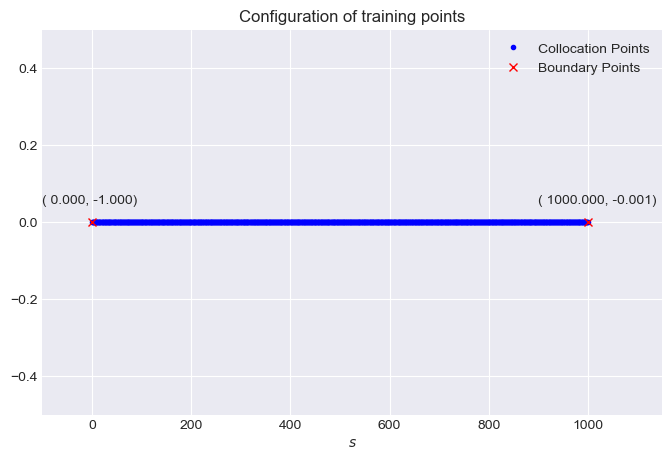
\includegraphics[width=\textwidth]{imgs/training-points-hernquist.png}
        \caption{Configuration of training points in the spatial domain $s \in [0, 1000]$.}
        \label{fig:training-points-hernquist}
    \end{figure}
    \column{\moit}
    \begin{figure}
        \centering
        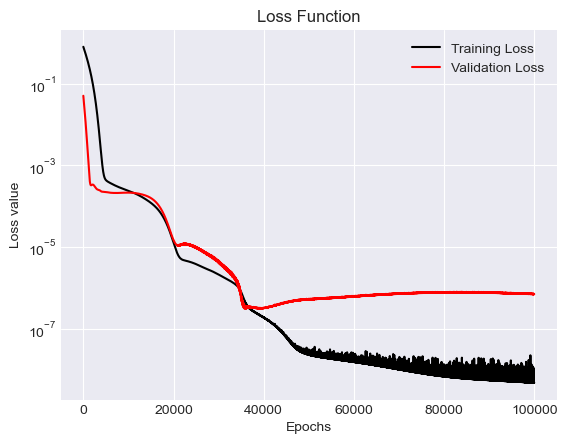
\includegraphics[width=\textwidth]{imgs/error-hernquist.png}
        \caption{Evolution of training and validation error functions.}
        \label{fig:losses-hernquist}
    \end{figure}
\end{columns}
\end{frame}

\begin{frame}{Hernquist - Results}

\begin{figure}
    \centering
        \begin{subfigure}[b]{0.49\textwidth}
        \centering
        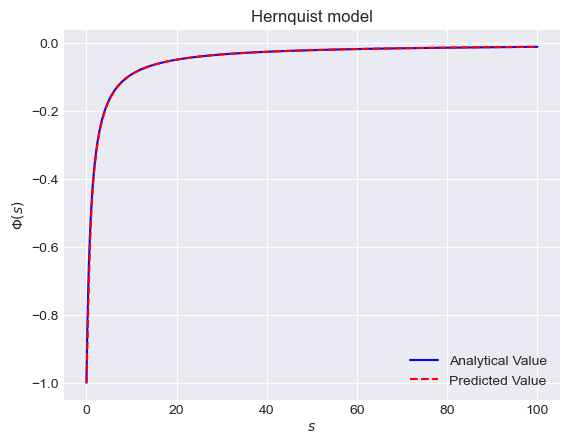
\includegraphics[width=\textwidth]{imgs/test-plot-hernquist.png}
        \caption{Comparison between the actual value of the potential and that predicted by the PINN on a test domain $s \in [0, 100]$.}
        \label{fig:test-plot-hernquist}
        \end{subfigure}
    \hfill
    \begin{subfigure}[b]{0.49\textwidth}
        \centering
        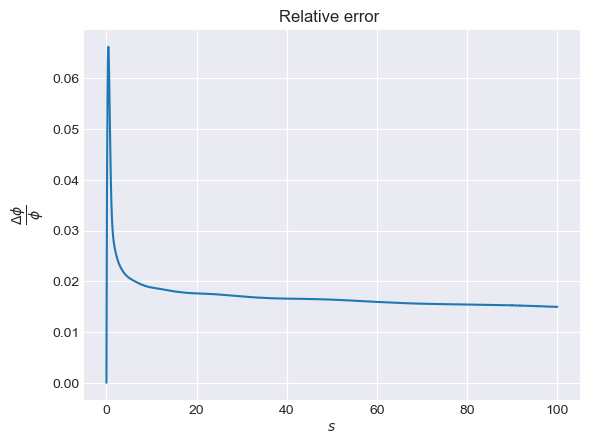
\includegraphics[width=\textwidth]{imgs/relative-error-hernquist.png}
        \caption{Relative error along the domain $s$. The average error over the entire domain is $1.71$\%.}
        \label{fig:relative-error-hernquist}
    \end{subfigure}
    \caption{As illustrated by the two figures presented, a PINN is capable of predicting with acceptable accuracy the value of the Hernquist potential $\Phi$ at a given point in a domain in which it has been trained.}
    \label{fig:three graphs}
\end{figure}
\end{frame}


\begin{frame}{Dehnen Model}
\only<1>{The differential equation we want to solve:

\begin{equation*}
    \dfrac{\dd}{\dd s}\left(s^2 \dfrac{\dd \Phi'}{\dd s}\right) = \dfrac{2s^{2-\gamma}}{(1+s)^{4-\gamma}}
\end{equation*}}

The exponent $\gamma$ drastically changes the dynamics of the potential:
\only<2>{
\begin{figure}
\centering
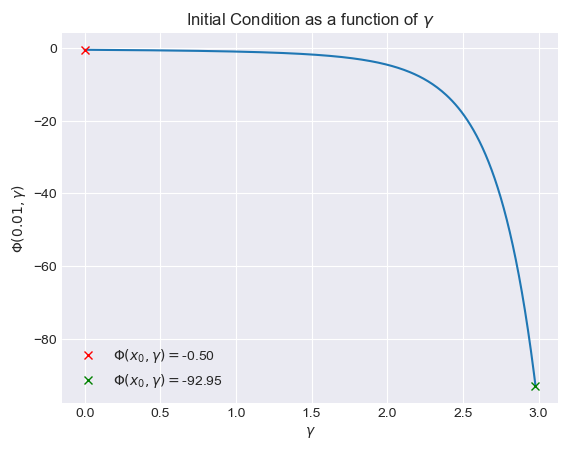
\includegraphics[width=0.6\textwidth]{imgs/gamma-vs-x0-dehnen.png}
\caption{Value of the gravitational potential at $s_0 = 0.01$ for different values of $\gamma \in [0, 3[$. Predicting the potential value at $s_0=0$ is a complex task for the PINN given the high sensitivity of $\Phi(s_0, \gamma)$ to the value of $\gamma$.}
\label{fig:gamma-vs-x0-dehnen}
\end{figure}}
\end{frame}
\subsection{Dehnen Model}\label{sec:dehnen}


\begin{frame}{Dehnen - Training}
    \begin{columns}
        \column{\moit} \begin{figure}
            \centering
            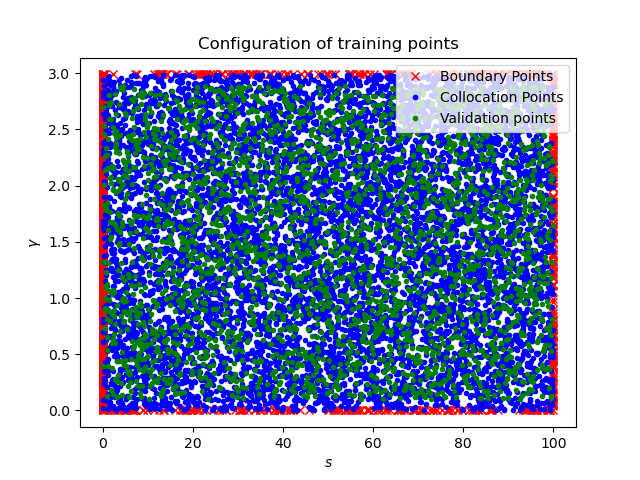
\includegraphics[width=\textwidth]{imgs/training-points-dehnen.png}
            \caption{Distribution of training and validation points on the domain.}
            \label{fig:training-points-dehnen}
        \end{figure}
        \column{\moit} \begin{itemize}
            \item Problems to obtain satisfactory results
            \item No observable improvement by manually tuning hyperparameters
            \item Change the penality of loss function to MAE
        \end{itemize}
    \end{columns}
\end{frame}



\begin{frame}{Dehnen - Results}
    \begin{columns}
    \column{\moit}
        \begin{figure}
            \centering
            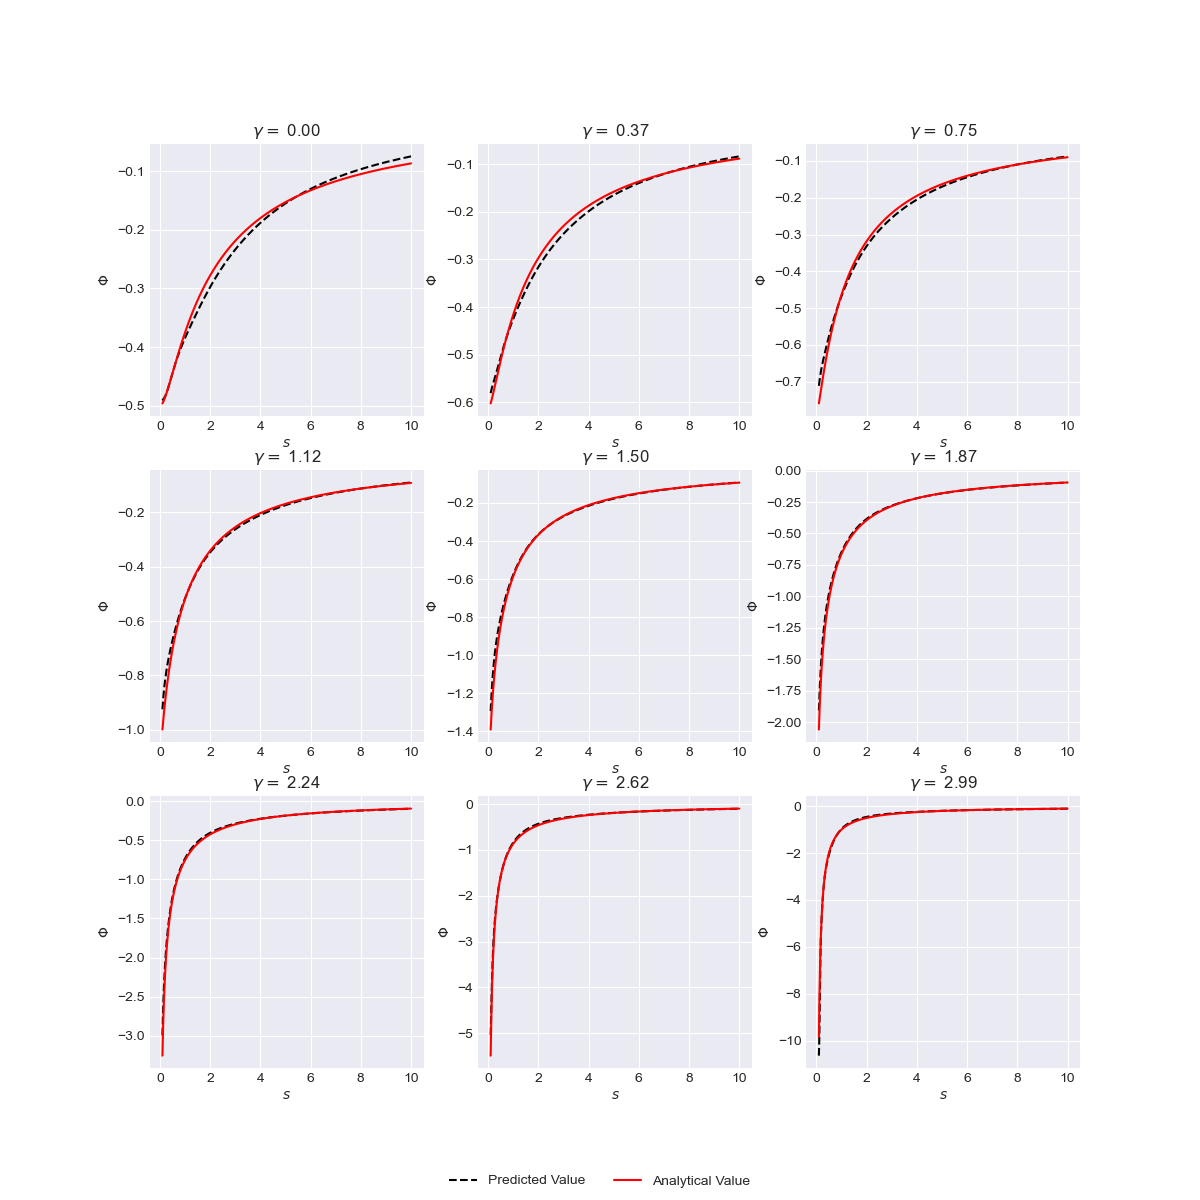
\includegraphics[width=\textwidth]{imgs/test-plot-dehnen.png}
            \caption{Comparison between the real value of the potential and that predicted by the PINN on a test domain $s \in [0, 10]$ for different values of $\gamma$.}
            \label{fig:test-plot-dehnen}
        \end{figure}
    \column{\moit} 
        \begin{figure}
            \centering
            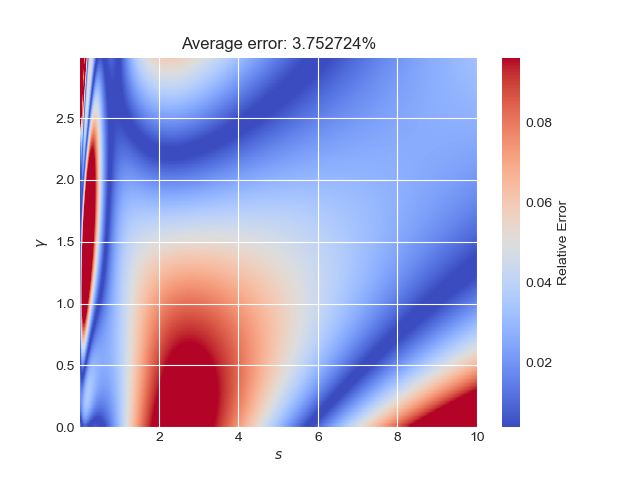
\includegraphics[width=\textwidth]{imgs/relative-error-dehnen.png}
            \caption{Relative error on the $s \times \gamma$ grid. The relative error can reach nearly 20\%.}
            \label{fig:relative-error-dehnen}
        \end{figure}
    \end{columns}
\end{frame}



\subsection{Thick Exponential Disk}\label{sec:disk}

\begin{frame}{Thick Exponential Disk Model}
    We aim to solve the following differential equation:
    \begin{equation*}
        \dfrac{1}{R'} \dfrac{\partial}{\partial R'} \left(R' \dfrac{\partial \Phi'}{\partial R'}\right) + \dfrac{1}{\eta^{2}}\dfrac{\partial^2 \Phi'}{\partial z'^2} = e^{-R'} \cosh^{-2}{z'}
\end{equation*} 
$z' = z/z_d$, $R' = R/R_d$, $\eta = z_d/R_d $ and $\phi'= \frac{\phi}{G M_d/z_d}$
\end{frame}

\begin{frame}{Thick Exponential Disk - Training}
    \begin{columns}
        \column{0.4\textwidth} 
        \begin{itemize}
            \item Wish to obtain the best solution possible
            \item Need to find the best set of hyperparameters
            \item Wish to understand the impact of certain hyperpameters on the error

        \end{itemize}
        \column{0.6\textwidth}
        Simple grid search for hyperparameters fine-tuning
        \begin{table}[h]
        \centering
        \scalebox{0.8}{
        \begin{tabular}{|l|c|}
        \hline
        \textbf{Parameters} & \textbf{Values} \\
            \hline
            \# Neurons & 32, 64, 128 \\
            \hline
            \# Layers & 1, 2, 3, 4, 5, 6 \\
            \hline
            Learning Rate & 1e-4, 1e-5, 1e-6 \\
            \hline
            Loss Func. & mse \\
            \hline
            Activation & Tanh, Sigmoid, SiLU, LogSigmoid \\
            \hline
        \end{tabular}}
        \label{tab:fine-tuning}
        \end{table}
    \end{columns}
\end{frame}

\begin{frame}{Thick Exponential Disk - Results}
    \only<1>{
    Two kind of solutions:
    \begin{enumerate}
        \item Computing an approximate solution efficiently $\rightarrow 3 \times 32$ NN, ~ 80 seconds of computation and average error of $1.85\%$.
        \item Find a model giving the smallest error possible $\rightarrow$ fine-tuning, $6 \times 128$ NN, ~ 20 minutes of training and average error of $0.36\%$.
    \end{enumerate}}
    \only<2>{
    \begin{figure}
        \centering
        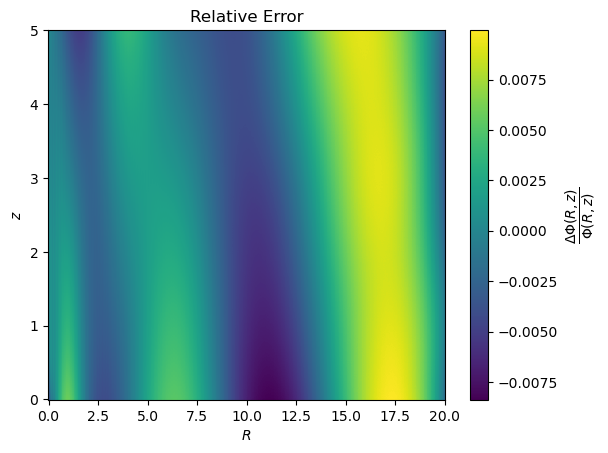
\includegraphics[width=0.6\textwidth]{imgs/relative-error-expdisc.png}
        %\caption{Relative error on the $R' \times z'$ grid. The average error over the entire domain is 0.36\%, and the maximum error is 0.99\%.}
        \label{fig:relative-error-expdisc}
    \end{figure}
    Satisfactory result, but parameter $\eta$ is here fixed $\rightarrow$ Need to extend the PINN !
    }
    
\end{frame}

\begin{frame}{Hyperparameters}
    How do hyper-parameters influence the relative error? 
    \only<1>{The activation function:
    \begin{figure}
        \centering
        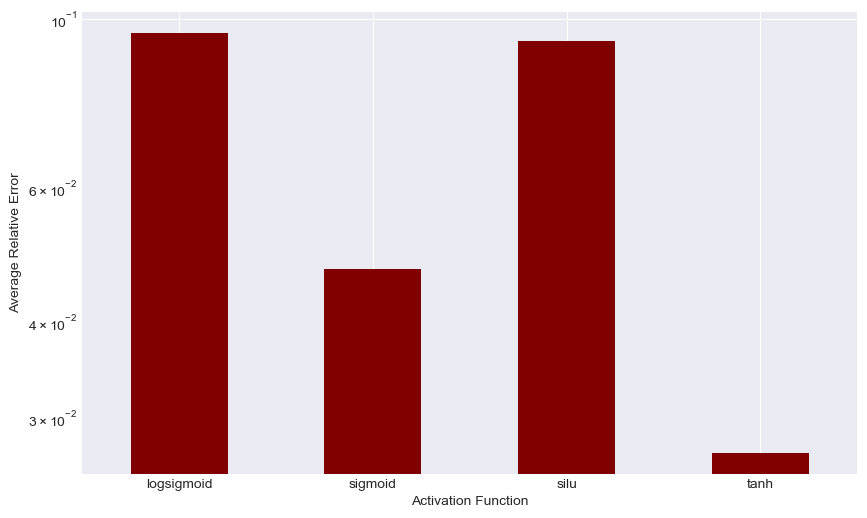
\includegraphics[scale=0.5]{imgs/function-error-expdisc.png}
        %\caption{Average relative error for certain activation functions.}
        \label{fig:function-error-expdisc}
    \end{figure}
}
    \only<2>{The learning rate:
    \begin{figure}
        \centering
        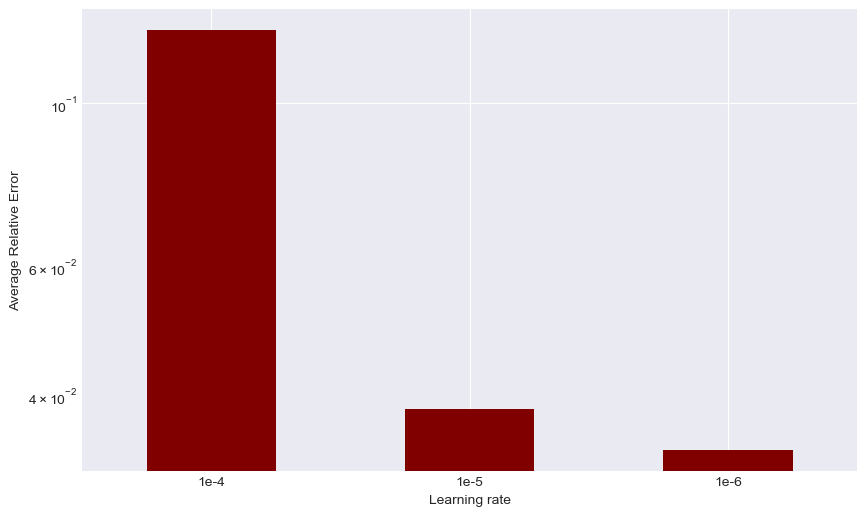
\includegraphics[scale=0.5]{imgs/learning-rate-expdisc.png}
        %\caption{Average relative error for different learning rates.}
        \label{fig:learning-rate-expdisc}
    \end{figure}
    }

    \only<3>{The number of neurons per layer:
     \begin{figure}
        \centering
        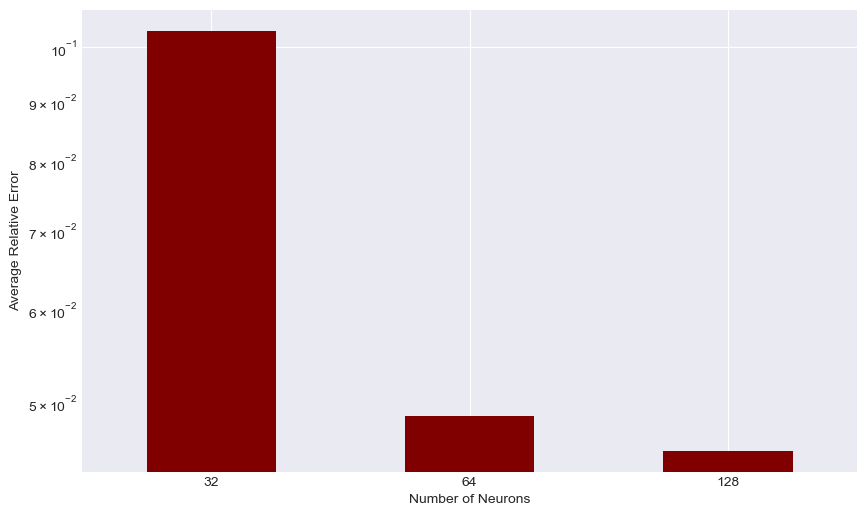
\includegraphics[scale=0.4]{imgs/neurons-error-expdisc.png}
        %\caption{Influence of the number of neurons per hidden layer on the average relative error.}
        %\label{fig:neurons-error-expdisc}
    \end{figure}
    }
    \only<4>{The number of hidden layers:
    \begin{figure}
        \centering
        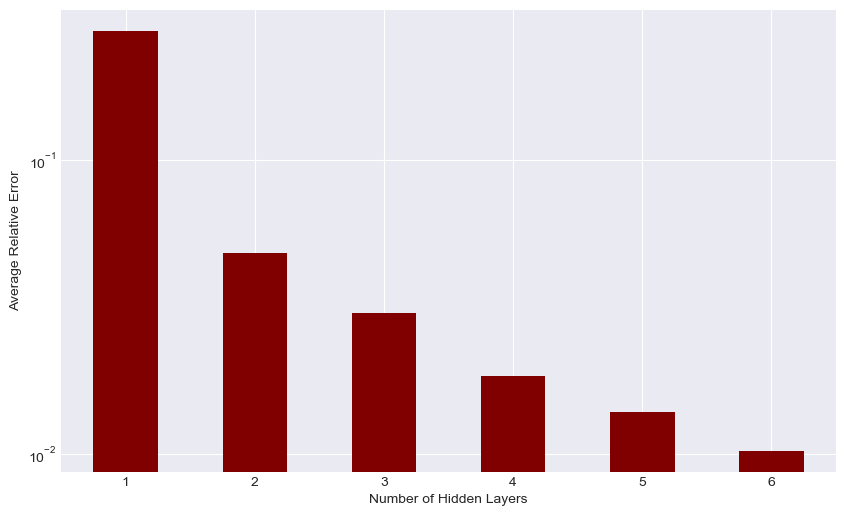
\includegraphics[scale=0.4]{imgs/layers-error-expdisc.png}
        %\caption{Influence of the number of hidden layers on the average relative error.}
        %\label{fig:layers-error-expdisc}
        \end{figure}
    }
    \only<5>{Is it solely the total number of neurons, or does the architecture have an impact?
    \begin{figure}
        \centering
        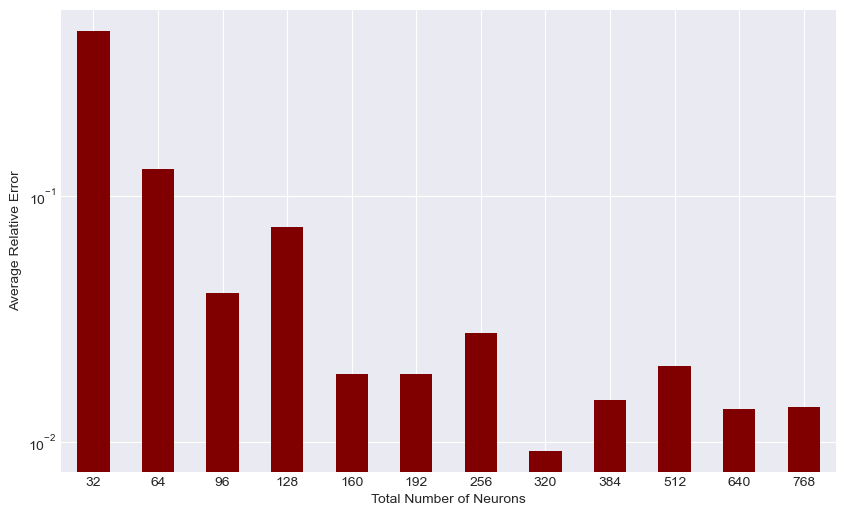
\includegraphics[width=0.65\textwidth]{imgs/tot-neurons-error.png}
        %\caption{Evolution of the average relative error as a function of the total number of neurons in the PINNs.}
        \label{fig:tot-neurons-error}
    \end{figure}
    }
\end{frame}

